% Options for packages loaded elsewhere
\PassOptionsToPackage{unicode}{hyperref}
\PassOptionsToPackage{hyphens}{url}
\documentclass[
]{article}
\usepackage{xcolor}
\usepackage[margin=1in]{geometry}
\usepackage{amsmath,amssymb}
\setcounter{secnumdepth}{-\maxdimen} % remove section numbering
\usepackage{iftex}
\ifPDFTeX
  \usepackage[T1]{fontenc}
  \usepackage[utf8]{inputenc}
  \usepackage{textcomp} % provide euro and other symbols
\else % if luatex or xetex
  \usepackage{unicode-math} % this also loads fontspec
  \defaultfontfeatures{Scale=MatchLowercase}
  \defaultfontfeatures[\rmfamily]{Ligatures=TeX,Scale=1}
\fi
\usepackage[]{bera}
\ifPDFTeX\else
  % xetex/luatex font selection
\fi
% Use upquote if available, for straight quotes in verbatim environments
\IfFileExists{upquote.sty}{\usepackage{upquote}}{}
\IfFileExists{microtype.sty}{% use microtype if available
  \usepackage[]{microtype}
  \UseMicrotypeSet[protrusion]{basicmath} % disable protrusion for tt fonts
}{}
\makeatletter
\@ifundefined{KOMAClassName}{% if non-KOMA class
  \IfFileExists{parskip.sty}{%
    \usepackage{parskip}
  }{% else
    \setlength{\parindent}{0pt}
    \setlength{\parskip}{6pt plus 2pt minus 1pt}}
}{% if KOMA class
  \KOMAoptions{parskip=half}}
\makeatother
\usepackage{color}
\usepackage{fancyvrb}
\newcommand{\VerbBar}{|}
\newcommand{\VERB}{\Verb[commandchars=\\\{\}]}
\DefineVerbatimEnvironment{Highlighting}{Verbatim}{commandchars=\\\{\}}
% Add ',fontsize=\small' for more characters per line
\usepackage{framed}
\definecolor{shadecolor}{RGB}{248,248,248}
\newenvironment{Shaded}{\begin{snugshade}}{\end{snugshade}}
\newcommand{\AlertTok}[1]{\textcolor[rgb]{0.94,0.16,0.16}{#1}}
\newcommand{\AnnotationTok}[1]{\textcolor[rgb]{0.56,0.35,0.01}{\textbf{\textit{#1}}}}
\newcommand{\AttributeTok}[1]{\textcolor[rgb]{0.13,0.29,0.53}{#1}}
\newcommand{\BaseNTok}[1]{\textcolor[rgb]{0.00,0.00,0.81}{#1}}
\newcommand{\BuiltInTok}[1]{#1}
\newcommand{\CharTok}[1]{\textcolor[rgb]{0.31,0.60,0.02}{#1}}
\newcommand{\CommentTok}[1]{\textcolor[rgb]{0.56,0.35,0.01}{\textit{#1}}}
\newcommand{\CommentVarTok}[1]{\textcolor[rgb]{0.56,0.35,0.01}{\textbf{\textit{#1}}}}
\newcommand{\ConstantTok}[1]{\textcolor[rgb]{0.56,0.35,0.01}{#1}}
\newcommand{\ControlFlowTok}[1]{\textcolor[rgb]{0.13,0.29,0.53}{\textbf{#1}}}
\newcommand{\DataTypeTok}[1]{\textcolor[rgb]{0.13,0.29,0.53}{#1}}
\newcommand{\DecValTok}[1]{\textcolor[rgb]{0.00,0.00,0.81}{#1}}
\newcommand{\DocumentationTok}[1]{\textcolor[rgb]{0.56,0.35,0.01}{\textbf{\textit{#1}}}}
\newcommand{\ErrorTok}[1]{\textcolor[rgb]{0.64,0.00,0.00}{\textbf{#1}}}
\newcommand{\ExtensionTok}[1]{#1}
\newcommand{\FloatTok}[1]{\textcolor[rgb]{0.00,0.00,0.81}{#1}}
\newcommand{\FunctionTok}[1]{\textcolor[rgb]{0.13,0.29,0.53}{\textbf{#1}}}
\newcommand{\ImportTok}[1]{#1}
\newcommand{\InformationTok}[1]{\textcolor[rgb]{0.56,0.35,0.01}{\textbf{\textit{#1}}}}
\newcommand{\KeywordTok}[1]{\textcolor[rgb]{0.13,0.29,0.53}{\textbf{#1}}}
\newcommand{\NormalTok}[1]{#1}
\newcommand{\OperatorTok}[1]{\textcolor[rgb]{0.81,0.36,0.00}{\textbf{#1}}}
\newcommand{\OtherTok}[1]{\textcolor[rgb]{0.56,0.35,0.01}{#1}}
\newcommand{\PreprocessorTok}[1]{\textcolor[rgb]{0.56,0.35,0.01}{\textit{#1}}}
\newcommand{\RegionMarkerTok}[1]{#1}
\newcommand{\SpecialCharTok}[1]{\textcolor[rgb]{0.81,0.36,0.00}{\textbf{#1}}}
\newcommand{\SpecialStringTok}[1]{\textcolor[rgb]{0.31,0.60,0.02}{#1}}
\newcommand{\StringTok}[1]{\textcolor[rgb]{0.31,0.60,0.02}{#1}}
\newcommand{\VariableTok}[1]{\textcolor[rgb]{0.00,0.00,0.00}{#1}}
\newcommand{\VerbatimStringTok}[1]{\textcolor[rgb]{0.31,0.60,0.02}{#1}}
\newcommand{\WarningTok}[1]{\textcolor[rgb]{0.56,0.35,0.01}{\textbf{\textit{#1}}}}
\usepackage{graphicx}
\makeatletter
\newsavebox\pandoc@box
\newcommand*\pandocbounded[1]{% scales image to fit in text height/width
  \sbox\pandoc@box{#1}%
  \Gscale@div\@tempa{\textheight}{\dimexpr\ht\pandoc@box+\dp\pandoc@box\relax}%
  \Gscale@div\@tempb{\linewidth}{\wd\pandoc@box}%
  \ifdim\@tempb\p@<\@tempa\p@\let\@tempa\@tempb\fi% select the smaller of both
  \ifdim\@tempa\p@<\p@\scalebox{\@tempa}{\usebox\pandoc@box}%
  \else\usebox{\pandoc@box}%
  \fi%
}
% Set default figure placement to htbp
\def\fps@figure{htbp}
\makeatother
\setlength{\emergencystretch}{3em} % prevent overfull lines
\providecommand{\tightlist}{%
  \setlength{\itemsep}{0pt}\setlength{\parskip}{0pt}}
\usepackage{bookmark}
\IfFileExists{xurl.sty}{\usepackage{xurl}}{} % add URL line breaks if available
\urlstyle{same}
% fallback for those not using the hyperref driver hyperxmp:
\makeatletter
\@ifundefined{xmpquote}{\newcommand{\xmpquote}[1]{#1}}{}
\makeatother
\hypersetup{
  pdftitle={Solutions to Introductory Quiz in Probability},
  pdfauthor={Vassilis Markos},
  hidelinks,
  pdfcreator={LaTeX via pandoc}}

\title{Solutions to Introductory Quiz in Probability}
\author{Vassilis Markos}
\date{}

\begin{document}
\maketitle
\begin{abstract}
Solutions to last time's introductory quiz with brief comments for each
one. Also, do not miss the minor challenges in some of the most (or
least) interesting questions!
\end{abstract}

\section{Question 1}\label{question-1}

\begin{quote}
We toss a fair coin three times. The probability of HHH (three times
``heads'') is less than the probability of HTH (``heads'', followed by
``tails'', followed by ``head'').
\end{quote}

\textbf{True.} This is a relatively simple question on classical
probability. Simple counting works miracles here, since there is just
one event where all tosses yield H, and there is also exactly one series
of tossses resulting to HTH, so the two probabilities must be equal
(given the fairness of the used coin).

In particular, the corresponding probability is: \(\frac{1}{8}\).

\section{Question 2}\label{question-2}

\begin{quote}
We toss a fair coin three times. The probability of seeing H twice is
greater than the probability of seeing H trice.
\end{quote}

\textbf{True.} Again, this boils down to simple counting. There is only
one event where we have HHH (HHH itself), while there are three events
where we encounter exactly two heads, namely: HHT, HTH, THH. So, since
\(3>1\), there are more chances to see H twice than trice.

\emph{Twist:} What if we tossed the coin 5 times? Is seeing H twice or
trice the most possible outcome?

\section{Question 3}\label{question-3}

\begin{quote}
We roll two fair dices. What is the probability of both dices bringing
the same result?
\end{quote}

The correct answer is \(\frac{1}{6}\) as most of you have correctly
responded. The total number of combinations is \(6\cdot 6=36\), while
those of interest are exactly \(6\) (both dices facing up the same
value). So, in total, we have:

\[\frac{6}{36}=\frac{1}{6}.\]

\section{Question 4}\label{question-4}

\begin{quote}
In a multiple choice test each question has 4 possible answer, with
exactly one of those being correct. A particular participant knows the
correct answer in a question with probability 0.70. Then, the
probability of knowing the answer having answered correctly is\ldots{}
\end{quote}

The correct answer is \(0.90\). The easiest way to see this is by using
conditional probabilities, so, let \(A\) be the event that the can
answer correctly and \(B\) the event that the student answers correctly.
In that setting, we already know that \(p(A)=0.70\) and we are
interested in \(p(A\mid B)\). From the Total Probability Theorem (which
is no more than just partitioning the event space) we get:

\[p(B)=p(B\cap A)+p(B\cap A')=p(B\mid A)p(A)+p(B\mid A')p(A').\]

So, the probability of the student answering correctly in a question
they do know (\(B\cap A\)) is \(0.70\), as we already know, while the
probability they answer correctly a question they do not know is
\(\frac{1}{4}\times 0.30=0.075\). So, in total:

\[p(B)=0.70+0.075=0.775.\]

Then, we have:

\[p(A\mid B)=\frac{p(A\cap B)}{p(B)}=\frac{0.70}{0.775}\approx0.90.\]

\subsection{Another line of
attack\ldots{}}\label{another-line-of-attack}

We can also answer the above by counting. The percentage of questions
answered correctly will be \(70\%\) plus one fourth of the other
\(30\%\) the student cannot answer correctly, so they answer at random.
That is, the percentage of the correctly answered questions is roughly
\(77.5\%\), out of which the student knows the answer in \(70/77.5\)
questions, which is the same ratio as the one we obtained above. So,
even if you were not aware of conditional probabilities and Bayes'
formula, you could work things out using just\ldots{} counting!

\section{Question 5}\label{question-5}

\begin{quote}
We toss a fair coin 4 times. What is the probability of getting 3 times
H and one time T?
\end{quote}

The correct answer is \(\frac{1}{4}\). Indeed, in order to get 3 H and 1
T we have four possible combinations, depending on the position at which
T appears (1st, 2nd, 3rd or 4th). So, 4 out of the \(2^4=16\) possible
outcomes in total, i.e.:

\[\frac{4}{16}=\frac{1}{4}.\]

\section{Question 6}\label{question-6}

\begin{quote}
We toss a ``soft'' coin twice. The first time, the coin behaves as a
typical fair coin, while the second, if the result is H, then the
probability of getting again H is 0.70, but if it is T, then the
probability of getting again H is 0.40. What is the probability of
getting one H and one T in those two tosses?
\end{quote}

The correct answer is \(0.35\). Indeed, we have to discriminate between
the two results the first toss yields. So, let \(H_i,T_i\) be the events
of Heads / Tails in the \(i\)-th toss, respectively, for \(i=1,2\) and
\(H,T\) being the events of getting one time Heads / Tails repsectively.
So, we are interested in the probability:

\[p(HT)=p(H_1T_2)+p(H_2T_1).\]

We can compute this in each case by taking into account the coin's
softness, as follows:

\begin{itemize}
\tightlist
\item
  In the case the first toss is H, which happens with probability
  \(p(H_1)=0.50\), we then get T with probaiblity \(p(T_2)=0.30\), so we
  get \(p(H_1T_2)=0.50\cdot 0.30=0.15\).
\item
  Similarly, in case the first toss is T, with probability
  \(p(T_1)=0.50\), then we get \(H\) with probability \(p(H_2)=0.40\),
  so \(p(T_1H_2)=0.50\cdot0.40=0.20\).
\end{itemize}

In total, we obtain \(p(HT)=0.15+0.20=0.35\) as promised.

\section{Question 7}\label{question-7}

\begin{quote}
The intersection of two sets A, B, corresponds to the set of all
elements belonging to both A and B.
\end{quote}

\textbf{True}, by the very definition of the intersection, \(A\cap B\)
of two sets.

\section{Question 8}\label{question-8}

\begin{quote}
The union of two sets A, B, corresponds to the set of all elements
belonging either to A or B but not both.
\end{quote}

\textbf{True}, again by the definition of \(A\cup B\). Observe that in
set theory, the union always includes the intersection of the same two
sets, i.e.:

\[A\cap B\subseteq A\cup B\]

which might contradict the common everyday use of ``or'' as
``either\ldots{} or\ldots{}''. Bear this in mind as you formulate
problems from natural language to mathematics.

\section{Question 9}\label{question-9}

\begin{quote}
The average height of a football team is 1.76. Selling a player of
height 1.83 and buying a player of height 1.81 will\ldots{}
\end{quote}

\textbf{lower the team's average height.} This is expected, since we
remove a larger observation from our sample than the one we introduce.
In particular, taking some time to do the math, let \(S\) denote the sum
of heights of the \(n\) players of the team. Then, the new total height
will be given by:

\[S'=S-1.83+1.82=S-0.02,\]

so the new average value will be:

\[\mu'=\frac{S'}{n}=\frac{S-0.02}{n}=\frac{S}{n}-\frac{0.02}{n}<\frac{S}{n}=\mu.\]

So, indeed, \(\mu'<\mu\).

\section{Question 10}\label{question-10}

\begin{quote}
Let X be a sample of 37 observations with mean value 23. Multiplying all
sample observations by -3, the new average will be\ldots{}
\end{quote}

\textbf{-69.} It is a given fact that the mean value is sensitive to
linear transformations, i.e., that the mean value of \(aX+b\) equals
\(a\mu+b\) where \(\mu\) is the mean value of \(X\). Hence, in our case:

\[\mu'=-3\mu=-3\cdot23=-69.\]

\section{Question 11}\label{question-11}

\begin{quote}
Students of a Probability course score on average 13 points in a 0-20
scale, with a standard deviation of 5.84. Assuming we convert all grades
to a 0-100 scale, the standard corresponding mean value, \(\mu\), and
standard deviation, s, will be\ldots{}
\end{quote}

\(\mu=65,s=29.20\). As we discussed before, the mean value is sensitive
to linear transformations, while standard deviation is sensitive only to
scaling, i.e., if \(s\) is the standard deviation of a random variable
\(X\), then the standard deviaation of \(aX+b\) will be:

\[s'=|a|s.\]

\emph{As a piece of intuition, think of the sample as a piece of dough.
In this analogy, mean value corresponds to its centre of mass and
standard deviation to the distribution of the dough around its centre of
mass. Thus, moving the dough around naturally moves its centre of mass
(mean value) but does not affect its shape (standard deviation), while
if we scale the dough, then naturally its centred of mass is
appropriately scaled, e.g., when the dough puffs, while this is also
true for its shape, which is naturally affected by this transformation.}

\section{Question 12}\label{question-12}

\begin{quote}
In a sample of 183 observations, we add a new value equal to the maximum
observation in the sample. Which of the following statistical functions
is not guaranteed to increase?
\end{quote}

The \textbf{median} is, in general, the least vulnerable to extreme
observations since it captures the point in the sample which evenly
splits the sample. All other measures mentioned, given that they
involve, among others, both extreme observations, are naturally affected
by new extreme observations. For a demonstration, consider the following
sample of 7 observations:

\[1,1,2,4,4,7,8.\]

Then, adding another extreme value, e.g., \(2027\), will result to the
range, mean value and standard deviation increasing significantly (you
can verify this computationally), but the median remains intact at
\(\delta=4\) in both samples.

\section{Question 13}\label{question-13}

\begin{quote}
The mean value of sample is not sensitive to extreme observations.
\end{quote}

\textbf{False}, as illustrated by the previous example (see Question
12).

\section{Question 14}\label{question-14}

\begin{quote}
We choose two balls from a bowl containing 12 black and 8 white ones
without replacement. The probability of getting two balls of the same
colour is\ldots{}
\end{quote}

\textbf{192/380.} To see this, let us denote by \(B_i,W_i\) the events
of drawing a black and white ball at iteration \(i=1,2\), respectively.
Then, we are interested in the probability:

\[p(B_1W_2\cup W_1B_2)=p(B_1W_2)+p(W_1B_2).\]

Given that there is no replacement, i.e., each ball extracted is then
removed from the bowl, we easily get:

\[p(B_1W_2)=\frac{12}{20}\frac{8}{19}.\]

Similarly:

\[p(W_1B_2)=\frac{8}{20}\frac{12}{19}.\]

So, in total (\(BW\) denotes the event of interest, just for
simplicity):

\[p(BW)=\frac{12}{20}\frac{8}{19}+\frac{8}{20}\frac{12}{19}=\frac{192}{380}.\]

\emph{You might observe some symmetry between the two cases examined
above. Is this a generalisable observation or is it coincidental?}

\section{Question 15}\label{question-15}

\begin{quote}
We choose two balls from a bowl containing 12 black and 8 white ones
with replacement. The probability of getting two balls of the same
colour is\ldots{}
\end{quote}

\textbf{192/400.} The idea is identical to the previous question, just
taking into account that now that we replace balls into the bowl, all
denominators are equal to 20.

\section{Question 16}\label{question-16}

\begin{quote}
We choose two numbers (not necessarily different\}, x, y, uniformly at
random from the set \{1,2,\ldots,100\}. Then, their sum, x + y, is
uniformly distributed on the set \{2,3,\ldots,200\}.
\end{quote}

\textbf{False.} This is a classic in statistics / probability related
interviews, so\ldots{} heads up! Even if \(x,y\) are drawn from a
uniform distribution, i.e., completely at random, the distribution of
their sum is not uniform. To see this, observe that, e.g., \(x+y=2\) can
be obtained only through \(x=y=1\), while for \(x+y=100\) we have the
following combinations:

\[(x,y)\in\{(1,99),(2,98),\ldots,(99,1)\}.\]

In general, the distribution of \(x+y\) is what we refer to as
\emph{triangular} distribution, since the middle values can be obtained
with higher probability for combinatorial reasons.

\section{Question 17}\label{question-17}

\begin{quote}
A flu test is positive with probability 0.95 given that the patient is
actually sick, and with probability 0.20 if the patient is not actually
sick. In a population where about 3\% of the population is sick, what is
the probability that a person tests positive?
\end{quote}

\textbf{0.2225.} Let \(+\) and \(F\) be the events that a person tests
positive and that a person is down with the flu, respectively. Then, the
above data translate to:

\[P(+\mid F)=0.95,\quad P(+\mid F')=0.20\] and:

\[P(F)=0.03.\] Then, we are interested into computing the probability
\(P(+)\). We can think in terms of the Total Probability Theorem (or
just, by partitioning our population into people who are sick and people
who are not) as follows:

\[P(+)=P(+\cap F)+P(+\cap F'),\] i.e., the probability for one person to
test positive is the some of the probability of testing positive and
being sick plus the probability of testing positive and not being sick.
Given the above data, we have:

\[
\begin{aligned}
  P(+\cap F)&=P(+\mid F)P(F)=0.95\cdot0.03=0..0285\\
  P(+\cap F')&=P(+\mid F')P(F')=0.20\cdot0.97=0.194
\end{aligned}
\]

So, in total:

\[P(+)=0.0285+0.194=0.2225.\]

\section{Question 18}\label{question-18}

\begin{quote}
How many anagrams of the word ``grass'' are there?
\end{quote}

\textbf{60.} The word anagram might be of some confusion here. To create
an anagram of grass, we have out our disposal 1 `g', 1 `r', 1 `a' and 2
`s' and we are allowed to order them in a any way we wish two, not
distinguishing, of course, between copies of the same letter. So, we can
think of an anagram as a sequence of five letters where we have:

\begin{itemize}
\tightlist
\item
  five choices to place `g' (any of the five empty slots);
\item
  four choices to place `r' (since `g' now occupies one of the five
  slots);
\item
  three choices to place `a' (since `g' and `r' take up two slots), and;
\item
  one choice on where to place both `s', since we have been left with
  only two empty slots and we cannot distinguish between the two `s'
  characters.
\end{itemize}

This amounts to \(5\cdot4\cdot3\cdot1=60\) different choices.

\section{Question 19}\label{question-19}

\begin{quote}
The probability of a dice yielding an odd number is:
\end{quote}

\textbf{1/2.} This is easy to check as out the 6 values in
\(\{1,2,3,4,5,6\}\), there are exactly 3 that are odd, so the
probability of getting an odd result is:

\[p=\frac{3}{6}={1}{2}.\]

\section{Question 20}\label{question-20}

\begin{quote}
We inscribe an equilateral triangle in a circle and pick a chord of the
circle at random. What is the probability that the chord is longer than
the side of the equilateral triangle?
\end{quote}

\textbf{All of the above.} This was a trick question, as it corresponds
to the well known
\href{https://en.wikipedia.org/wiki/Bertrand_paradox_(probability)}{Bertrand
Paradox}. The problem, as stated above is unclear enough to allow for
different ways of computing the requested probability, thus yielding
different results.

\subsection{First Attempt}\label{first-attempt}

We can pick a chord at random by assuming that one of its edges
coincides with one of the three edges of the inscribed triangle and then
pick the other uniformly at random, as shown in the following Figure:

\begin{Shaded}
\begin{Highlighting}[]
\NormalTok{B }\OtherTok{=} \FloatTok{1.0}
\FunctionTok{plot}\NormalTok{(}\FunctionTok{c}\NormalTok{(), }\AttributeTok{axes=}\ConstantTok{FALSE}\NormalTok{, }\AttributeTok{ann=}\ConstantTok{FALSE}\NormalTok{, }\AttributeTok{xlim =} \FunctionTok{c}\NormalTok{(}\SpecialCharTok{{-}}\NormalTok{B,B), }\AttributeTok{ylim  =} \FunctionTok{c}\NormalTok{(}\SpecialCharTok{{-}}\NormalTok{B, B), }\AttributeTok{asp =} \DecValTok{1}\NormalTok{)}
\NormalTok{theta }\OtherTok{\textless{}{-}} \FunctionTok{seq}\NormalTok{(}\DecValTok{0}\NormalTok{, }\DecValTok{2} \SpecialCharTok{*}\NormalTok{ pi, }\AttributeTok{length.out =} \DecValTok{200}\NormalTok{) }\CommentTok{\# Values to be used for drawing}
\FunctionTok{lines}\NormalTok{(}\FunctionTok{cos}\NormalTok{(theta), }\FunctionTok{sin}\NormalTok{(theta))}
\CommentTok{\# Triangle edges}
\NormalTok{tth }\OtherTok{\textless{}{-}} \FunctionTok{c}\NormalTok{(}\DecValTok{0}\NormalTok{, }\DecValTok{2}\SpecialCharTok{*}\NormalTok{pi}\SpecialCharTok{/}\DecValTok{3}\NormalTok{, }\DecValTok{4}\SpecialCharTok{*}\NormalTok{pi}\SpecialCharTok{/}\DecValTok{3}\NormalTok{, }\DecValTok{2}\SpecialCharTok{*}\NormalTok{pi)}
\NormalTok{triangle.x }\OtherTok{\textless{}{-}} \FunctionTok{cos}\NormalTok{(tth)}
\NormalTok{triangle.y }\OtherTok{\textless{}{-}} \FunctionTok{sin}\NormalTok{(tth)}
\FunctionTok{lines}\NormalTok{(triangle.x, triangle.y)}
\CommentTok{\# Draw a single triangle edge}
\NormalTok{a.x }\OtherTok{\textless{}{-}} \DecValTok{1}
\NormalTok{a.y }\OtherTok{\textless{}{-}} \DecValTok{0}
\FunctionTok{points}\NormalTok{(}\AttributeTok{x =}\NormalTok{ a.x, }\AttributeTok{y =}\NormalTok{ a.y, }\AttributeTok{pch =} \DecValTok{19}\NormalTok{, }\AttributeTok{col =} \StringTok{"black"}\NormalTok{)}
\CommentTok{\# Draw some chords around the circle}
\NormalTok{th }\OtherTok{\textless{}{-}} \FunctionTok{seq}\NormalTok{(}\DecValTok{15}\NormalTok{, }\DecValTok{345}\NormalTok{, }\DecValTok{30}\NormalTok{) }\CommentTok{\# angles of 15, 45, ..., 345 degrees}
\NormalTok{xs }\OtherTok{\textless{}{-}} \FunctionTok{cos}\NormalTok{(th)}
\NormalTok{ys }\OtherTok{\textless{}{-}} \FunctionTok{sin}\NormalTok{(th)}
\FunctionTok{points}\NormalTok{(}\AttributeTok{x =}\NormalTok{ xs, }\AttributeTok{y =}\NormalTok{ ys, }\AttributeTok{pch =} \DecValTok{19}\NormalTok{, }\AttributeTok{col=}\StringTok{"coral"}\NormalTok{)}
\ControlFlowTok{for}\NormalTok{ (i }\ControlFlowTok{in} \DecValTok{1}\SpecialCharTok{:}\FunctionTok{length}\NormalTok{(xs)) \{}
  \FunctionTok{lines}\NormalTok{(}\FunctionTok{c}\NormalTok{(a.x, xs[i]), }\FunctionTok{c}\NormalTok{(a.y, ys[i]), }\AttributeTok{col=}\StringTok{"coral"}\NormalTok{)}
\NormalTok{\}}
\end{Highlighting}
\end{Shaded}

\pandocbounded{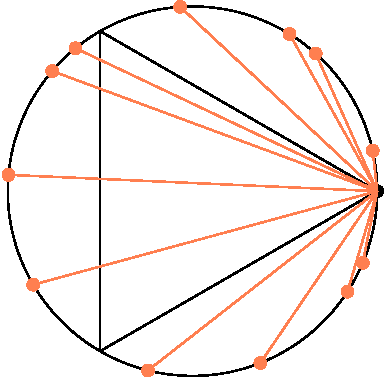
\includegraphics[keepaspectratio]{quiz_solutions_files/figure-latex/unnamed-chunk-1-1.pdf}}
So, a chord in this case is larger than the side of the equilateral
triangle exactly when the coloured edge falls into the coloured circular
arc shown below:

\begin{Shaded}
\begin{Highlighting}[]
\NormalTok{B }\OtherTok{=} \FloatTok{1.0}
\FunctionTok{plot}\NormalTok{(}\FunctionTok{c}\NormalTok{(), }\AttributeTok{axes=}\ConstantTok{FALSE}\NormalTok{, }\AttributeTok{ann=}\ConstantTok{FALSE}\NormalTok{, }\AttributeTok{xlim =} \FunctionTok{c}\NormalTok{(}\SpecialCharTok{{-}}\NormalTok{B,B), }\AttributeTok{ylim  =} \FunctionTok{c}\NormalTok{(}\SpecialCharTok{{-}}\NormalTok{B, B), }\AttributeTok{asp =} \DecValTok{1}\NormalTok{)}
\NormalTok{theta }\OtherTok{\textless{}{-}} \FunctionTok{seq}\NormalTok{(}\DecValTok{0}\NormalTok{, }\DecValTok{2} \SpecialCharTok{*}\NormalTok{ pi, }\AttributeTok{length.out =} \DecValTok{200}\NormalTok{) }\CommentTok{\# Values to be used for drawing}
\NormalTok{large }\OtherTok{\textless{}{-}}\NormalTok{ theta[theta }\SpecialCharTok{\textgreater{}} \DecValTok{2}\SpecialCharTok{*}\NormalTok{pi}\SpecialCharTok{/}\DecValTok{3} \SpecialCharTok{\&}\NormalTok{ theta }\SpecialCharTok{\textless{}} \DecValTok{4}\SpecialCharTok{*}\NormalTok{pi}\SpecialCharTok{/}\DecValTok{3}\NormalTok{]}
\NormalTok{small }\OtherTok{\textless{}{-}}\NormalTok{ theta[theta }\SpecialCharTok{\textless{}} \DecValTok{2}\SpecialCharTok{*}\NormalTok{pi}\SpecialCharTok{/}\DecValTok{3} \SpecialCharTok{|}\NormalTok{ theta }\SpecialCharTok{\textgreater{}} \DecValTok{4}\SpecialCharTok{*}\NormalTok{pi}\SpecialCharTok{/}\DecValTok{3}\NormalTok{]}
\FunctionTok{lines}\NormalTok{(}\FunctionTok{cos}\NormalTok{(small), }\FunctionTok{sin}\NormalTok{(small))}
\FunctionTok{lines}\NormalTok{(}\FunctionTok{cos}\NormalTok{(large), }\FunctionTok{sin}\NormalTok{(large), }\AttributeTok{col =} \StringTok{"coral"}\NormalTok{, }\AttributeTok{lwd =} \DecValTok{4}\NormalTok{)}
\CommentTok{\# Triangle edges}
\NormalTok{tth }\OtherTok{\textless{}{-}} \FunctionTok{c}\NormalTok{(}\DecValTok{0}\NormalTok{, }\DecValTok{2}\SpecialCharTok{*}\NormalTok{pi}\SpecialCharTok{/}\DecValTok{3}\NormalTok{, }\DecValTok{4}\SpecialCharTok{*}\NormalTok{pi}\SpecialCharTok{/}\DecValTok{3}\NormalTok{, }\DecValTok{2}\SpecialCharTok{*}\NormalTok{pi)}
\NormalTok{triangle.x }\OtherTok{\textless{}{-}} \FunctionTok{cos}\NormalTok{(tth)}
\NormalTok{triangle.y }\OtherTok{\textless{}{-}} \FunctionTok{sin}\NormalTok{(tth)}
\FunctionTok{lines}\NormalTok{(triangle.x, triangle.y)}
\CommentTok{\# Draw a single triangle edge}
\NormalTok{a.x }\OtherTok{\textless{}{-}} \DecValTok{1}
\NormalTok{a.y }\OtherTok{\textless{}{-}} \DecValTok{0}
\FunctionTok{points}\NormalTok{(}\AttributeTok{x =}\NormalTok{ a.x, }\AttributeTok{y =}\NormalTok{ a.y, }\AttributeTok{pch =} \DecValTok{19}\NormalTok{, }\AttributeTok{col =} \StringTok{"black"}\NormalTok{)}
\end{Highlighting}
\end{Shaded}

\pandocbounded{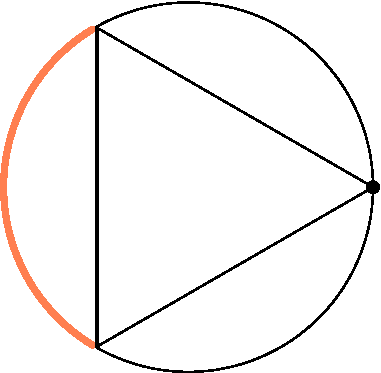
\includegraphics[keepaspectratio]{quiz_solutions_files/figure-latex/unnamed-chunk-2-1.pdf}}

\begin{Shaded}
\begin{Highlighting}[]
\CommentTok{\# }
\end{Highlighting}
\end{Shaded}

Given that all three arcs are of equal length, the requested probability
is \(p=1/3\).

\subsection{Second Attempt}\label{second-attempt}

Another way to randomly construct a chord in a circle is to pick its
midpoint at random, in which case, we have a situation like the one
shown below (picking all chord middle points on the same diameter just
for illustration purposes):

\begin{Shaded}
\begin{Highlighting}[]
\NormalTok{B }\OtherTok{=} \FloatTok{1.0}
\FunctionTok{plot}\NormalTok{(}\FunctionTok{c}\NormalTok{(), }\AttributeTok{axes=}\ConstantTok{FALSE}\NormalTok{, }\AttributeTok{ann=}\ConstantTok{FALSE}\NormalTok{, }\AttributeTok{xlim =} \FunctionTok{c}\NormalTok{(}\SpecialCharTok{{-}}\NormalTok{B,B), }\AttributeTok{ylim  =} \FunctionTok{c}\NormalTok{(}\SpecialCharTok{{-}}\NormalTok{B, B), }\AttributeTok{asp =} \DecValTok{1}\NormalTok{)}
\NormalTok{theta }\OtherTok{\textless{}{-}} \FunctionTok{seq}\NormalTok{(}\DecValTok{0}\NormalTok{, }\DecValTok{2} \SpecialCharTok{*}\NormalTok{ pi, }\AttributeTok{length.out =} \DecValTok{200}\NormalTok{) }\CommentTok{\# Values to be used for drawing}
\FunctionTok{lines}\NormalTok{(}\FunctionTok{cos}\NormalTok{(theta), }\FunctionTok{sin}\NormalTok{(theta))}
\CommentTok{\# Triangle edges}
\NormalTok{tth }\OtherTok{\textless{}{-}} \FunctionTok{c}\NormalTok{(}\DecValTok{0}\NormalTok{, }\DecValTok{2}\SpecialCharTok{*}\NormalTok{pi}\SpecialCharTok{/}\DecValTok{3}\NormalTok{, }\DecValTok{4}\SpecialCharTok{*}\NormalTok{pi}\SpecialCharTok{/}\DecValTok{3}\NormalTok{, }\DecValTok{2}\SpecialCharTok{*}\NormalTok{pi)}
\NormalTok{triangle.x }\OtherTok{\textless{}{-}} \FunctionTok{cos}\NormalTok{(tth)}
\NormalTok{triangle.y }\OtherTok{\textless{}{-}} \FunctionTok{sin}\NormalTok{(tth)}
\FunctionTok{lines}\NormalTok{(triangle.x, triangle.y)}
\CommentTok{\# Draw a single triangle edge}
\NormalTok{a.x }\OtherTok{\textless{}{-}} \DecValTok{1}
\NormalTok{a.y }\OtherTok{\textless{}{-}} \DecValTok{0}
\FunctionTok{points}\NormalTok{(}\AttributeTok{x =}\NormalTok{ a.x, }\AttributeTok{y =}\NormalTok{ a.y, }\AttributeTok{pch =} \DecValTok{19}\NormalTok{, }\AttributeTok{col =} \StringTok{"black"}\NormalTok{)}
\CommentTok{\# Draw flipped triangle for reference}
\NormalTok{ftth }\OtherTok{\textless{}{-}}\NormalTok{ pi }\SpecialCharTok{{-}}\NormalTok{ tth}
\NormalTok{ftriangle.x }\OtherTok{\textless{}{-}} \FunctionTok{cos}\NormalTok{(ftth)}
\NormalTok{ftriangle.y }\OtherTok{\textless{}{-}} \FunctionTok{sin}\NormalTok{(ftth)}
\FunctionTok{lines}\NormalTok{(ftriangle.x, ftriangle.y, }\AttributeTok{col =} \StringTok{"\#00000040"}\NormalTok{, }\AttributeTok{lty =} \StringTok{"dashed"}\NormalTok{)}
\CommentTok{\# Draw a diameter on which we place middle points}
\FunctionTok{lines}\NormalTok{(}\FunctionTok{c}\NormalTok{(a.x, }\SpecialCharTok{{-}}\DecValTok{1}\NormalTok{), }\FunctionTok{c}\NormalTok{(a.y, }\DecValTok{0}\NormalTok{))}
\CommentTok{\# Draw some chords}
\ControlFlowTok{for}\NormalTok{ (mx }\ControlFlowTok{in} \FunctionTok{seq}\NormalTok{(}\SpecialCharTok{{-}}\FloatTok{0.95}\NormalTok{, }\FloatTok{0.95}\NormalTok{, }\FloatTok{0.10}\NormalTok{)) \{}
\NormalTok{  my }\OtherTok{\textless{}{-}} \FunctionTok{sqrt}\NormalTok{(}\DecValTok{1} \SpecialCharTok{{-}}\NormalTok{ mx}\SpecialCharTok{\^{}}\DecValTok{2}\NormalTok{)}
\NormalTok{  colour }\OtherTok{\textless{}{-}} \StringTok{"coral"}
  \ControlFlowTok{if}\NormalTok{ (mx }\SpecialCharTok{\textgreater{}} \SpecialCharTok{{-}}\FloatTok{0.5} \SpecialCharTok{\&\&}\NormalTok{ mx }\SpecialCharTok{\textless{}} \FloatTok{0.5}\NormalTok{) \{}
\NormalTok{    colour }\OtherTok{\textless{}{-}} \StringTok{"turquoise"}
\NormalTok{  \}}
  \FunctionTok{lines}\NormalTok{(}\FunctionTok{c}\NormalTok{(mx, mx), }\FunctionTok{c}\NormalTok{(my, }\SpecialCharTok{{-}}\NormalTok{my), }\AttributeTok{col =}\NormalTok{ colour)}
  \FunctionTok{points}\NormalTok{(}\AttributeTok{x =}\NormalTok{ mx, }\AttributeTok{y =} \DecValTok{0}\NormalTok{, }\AttributeTok{pch =} \DecValTok{19}\NormalTok{, }\AttributeTok{col =}\NormalTok{ colour)}
\NormalTok{\}}
\end{Highlighting}
\end{Shaded}

\pandocbounded{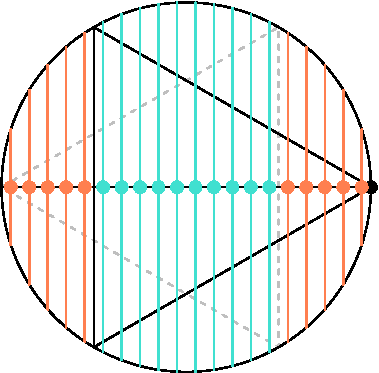
\includegraphics[keepaspectratio]{quiz_solutions_files/figure-latex/unnamed-chunk-3-1.pdf}}
By rotating the above figure we can easily see that all midpoints chosen
into the turquoise circle result to chords of length \textbf{less} than
the triangle's side while all midpoints in the coral coloured area
result to chords \textbf{greater} than the triangle's side.

\begin{Shaded}
\begin{Highlighting}[]
\NormalTok{B }\OtherTok{=} \FloatTok{1.0}
\FunctionTok{plot}\NormalTok{(}\FunctionTok{c}\NormalTok{(), }\AttributeTok{axes=}\ConstantTok{FALSE}\NormalTok{, }\AttributeTok{ann=}\ConstantTok{FALSE}\NormalTok{, }\AttributeTok{xlim =} \FunctionTok{c}\NormalTok{(}\SpecialCharTok{{-}}\NormalTok{B,B), }\AttributeTok{ylim  =} \FunctionTok{c}\NormalTok{(}\SpecialCharTok{{-}}\NormalTok{B, B), }\AttributeTok{asp =} \DecValTok{1}\NormalTok{)}
\NormalTok{theta }\OtherTok{\textless{}{-}} \FunctionTok{seq}\NormalTok{(}\DecValTok{0}\NormalTok{, }\DecValTok{2} \SpecialCharTok{*}\NormalTok{ pi, }\AttributeTok{length.out =} \DecValTok{200}\NormalTok{) }\CommentTok{\# Values to be used for drawing}
\FunctionTok{lines}\NormalTok{(}\FunctionTok{cos}\NormalTok{(theta), }\FunctionTok{sin}\NormalTok{(theta))}
\CommentTok{\# Triangle edges}
\NormalTok{tth }\OtherTok{\textless{}{-}} \FunctionTok{c}\NormalTok{(}\DecValTok{0}\NormalTok{, }\DecValTok{2}\SpecialCharTok{*}\NormalTok{pi}\SpecialCharTok{/}\DecValTok{3}\NormalTok{, }\DecValTok{4}\SpecialCharTok{*}\NormalTok{pi}\SpecialCharTok{/}\DecValTok{3}\NormalTok{, }\DecValTok{2}\SpecialCharTok{*}\NormalTok{pi)}
\NormalTok{triangle.x }\OtherTok{\textless{}{-}} \FunctionTok{cos}\NormalTok{(tth)}
\NormalTok{triangle.y }\OtherTok{\textless{}{-}} \FunctionTok{sin}\NormalTok{(tth)}
\FunctionTok{lines}\NormalTok{(triangle.x, triangle.y)}
\CommentTok{\# Draw a single triangle edge}
\NormalTok{a.x }\OtherTok{\textless{}{-}} \DecValTok{1}
\NormalTok{a.y }\OtherTok{\textless{}{-}} \DecValTok{0}
\FunctionTok{points}\NormalTok{(}\AttributeTok{x =}\NormalTok{ a.x, }\AttributeTok{y =}\NormalTok{ a.y, }\AttributeTok{pch =} \DecValTok{19}\NormalTok{, }\AttributeTok{col =} \StringTok{"black"}\NormalTok{)}
\CommentTok{\# Draw inner circle}
\NormalTok{r }\OtherTok{\textless{}{-}} \FloatTok{0.5}
\FunctionTok{polygon}\NormalTok{(r }\SpecialCharTok{*} \FunctionTok{cos}\NormalTok{(theta), r }\SpecialCharTok{*} \FunctionTok{sin}\NormalTok{(theta), }\AttributeTok{col =} \StringTok{"turquoise"}\NormalTok{, }\AttributeTok{lty =} \StringTok{"dashed"}\NormalTok{)}
\FunctionTok{polygon}\NormalTok{(}\FunctionTok{cos}\NormalTok{(theta), }\FunctionTok{sin}\NormalTok{(theta), }\AttributeTok{col =} \StringTok{"\#FF7F5050"}\NormalTok{)}
\end{Highlighting}
\end{Shaded}

\pandocbounded{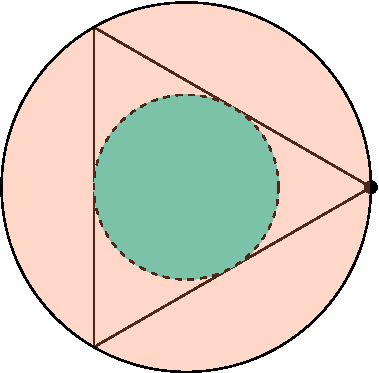
\includegraphics[keepaspectratio]{quiz_solutions_files/figure-latex/unnamed-chunk-4-1.pdf}}

This clearly results to probability (recalling that the area of a circle
is given by \(A=\pi r^2\)):

\[p=\frac{\pi(0.5)^2}{\pi1^2}=0.5^2=0.25=\frac{1}{4}.\]

\subsection{Third Attempt}\label{third-attempt}

Similarly to the above, we can pick a radius of the circle and draw a
chord on a random point of this radius as a perpendicular line to it
(each chord in a circle is uniquely determined by a radius and a point
on it). So, for example, we could draw something like the following:

\begin{Shaded}
\begin{Highlighting}[]
\NormalTok{B }\OtherTok{=} \FloatTok{1.0}
\FunctionTok{plot}\NormalTok{(}\FunctionTok{c}\NormalTok{(), }\AttributeTok{axes=}\ConstantTok{FALSE}\NormalTok{, }\AttributeTok{ann=}\ConstantTok{FALSE}\NormalTok{, }\AttributeTok{xlim =} \FunctionTok{c}\NormalTok{(}\SpecialCharTok{{-}}\NormalTok{B,B), }\AttributeTok{ylim  =} \FunctionTok{c}\NormalTok{(}\SpecialCharTok{{-}}\NormalTok{B, B), }\AttributeTok{asp =} \DecValTok{1}\NormalTok{)}
\NormalTok{theta }\OtherTok{\textless{}{-}} \FunctionTok{seq}\NormalTok{(}\DecValTok{0}\NormalTok{, }\DecValTok{2} \SpecialCharTok{*}\NormalTok{ pi, }\AttributeTok{length.out =} \DecValTok{200}\NormalTok{) }\CommentTok{\# Values to be used for drawing}
\FunctionTok{lines}\NormalTok{(}\FunctionTok{cos}\NormalTok{(theta), }\FunctionTok{sin}\NormalTok{(theta))}
\CommentTok{\# Triangle edges}
\NormalTok{tth }\OtherTok{\textless{}{-}} \FunctionTok{c}\NormalTok{(}\DecValTok{0}\NormalTok{, }\DecValTok{2}\SpecialCharTok{*}\NormalTok{pi}\SpecialCharTok{/}\DecValTok{3}\NormalTok{, }\DecValTok{4}\SpecialCharTok{*}\NormalTok{pi}\SpecialCharTok{/}\DecValTok{3}\NormalTok{, }\DecValTok{2}\SpecialCharTok{*}\NormalTok{pi)}
\NormalTok{triangle.x }\OtherTok{\textless{}{-}} \FunctionTok{cos}\NormalTok{(tth)}
\NormalTok{triangle.y }\OtherTok{\textless{}{-}} \FunctionTok{sin}\NormalTok{(tth)}
\FunctionTok{lines}\NormalTok{(triangle.x, triangle.y)}
\CommentTok{\# Draw a single triangle edge}
\NormalTok{a.x }\OtherTok{\textless{}{-}} \SpecialCharTok{{-}}\DecValTok{1}
\NormalTok{a.y }\OtherTok{\textless{}{-}} \DecValTok{0}
\FunctionTok{points}\NormalTok{(}\AttributeTok{x =}\NormalTok{ a.x, }\AttributeTok{y =}\NormalTok{ a.y, }\AttributeTok{pch =} \DecValTok{19}\NormalTok{, }\AttributeTok{col =} \StringTok{"black"}\NormalTok{)}
\CommentTok{\# Draw a radius}
\FunctionTok{lines}\NormalTok{(}\FunctionTok{c}\NormalTok{(}\DecValTok{0}\NormalTok{, }\SpecialCharTok{{-}}\DecValTok{1}\NormalTok{), }\FunctionTok{c}\NormalTok{(}\DecValTok{0}\NormalTok{, }\DecValTok{0}\NormalTok{))}
\CommentTok{\# Draw some chords}
\ControlFlowTok{for}\NormalTok{ (mx }\ControlFlowTok{in} \FunctionTok{seq}\NormalTok{(}\SpecialCharTok{{-}}\FloatTok{0.09}\NormalTok{, }\SpecialCharTok{{-}}\FloatTok{0.89}\NormalTok{, }\SpecialCharTok{{-}}\FloatTok{0.05}\NormalTok{)) \{}
\NormalTok{  my }\OtherTok{\textless{}{-}} \FunctionTok{sqrt}\NormalTok{(}\DecValTok{1} \SpecialCharTok{{-}}\NormalTok{ mx}\SpecialCharTok{\^{}}\DecValTok{2}\NormalTok{)}
\NormalTok{  colour }\OtherTok{\textless{}{-}} \StringTok{"turquoise"}
  \ControlFlowTok{if}\NormalTok{ (mx }\SpecialCharTok{\textgreater{}} \SpecialCharTok{{-}}\FloatTok{0.5}\NormalTok{) \{}
\NormalTok{    colour }\OtherTok{\textless{}{-}} \StringTok{"coral"}
\NormalTok{  \}}
  \FunctionTok{lines}\NormalTok{(}\FunctionTok{c}\NormalTok{(mx, mx), }\FunctionTok{c}\NormalTok{(my, }\SpecialCharTok{{-}}\NormalTok{my), }\AttributeTok{col =}\NormalTok{ colour)}
\NormalTok{\}}
\end{Highlighting}
\end{Shaded}

\pandocbounded{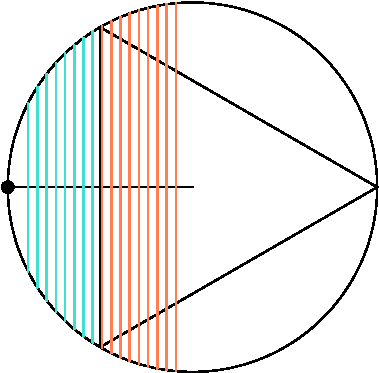
\includegraphics[keepaspectratio]{quiz_solutions_files/figure-latex/unnamed-chunk-5-1.pdf}}
As you might guess, the radius itself is of no importance, i.e., we can
rotate it arbitrarily. Also, observe that at the above figure the
triangle's side cutting the draw radius does so exactly at its middle
point, so half of the times, a randomly drawn chord will have length
greater than that side and half times it will not, i.e.:

\[p=\frac{1}{2}.\]

\subsection{So\ldots?}\label{so}

So far, we have seen that there are three different interpretations of
``randomly selecting a chord'' which result to three different results.
Which one should be the correct one? Well, there are various lines of
attack to this question but maybe the most straightforward would be to
see the corresponding distributions for each the above approaches, i.e.,
pick a large sample of random chords as per each approach and draw them,
trying to verify whether they disitribute uniformly on the unit disc. To
do so, we first create a utility function that draws a set of chords on
a unit circle:

\begin{Shaded}
\begin{Highlighting}[]
\CommentTok{\# \textasciigrave{}chords\textasciigrave{} is a list of lists of start end x and y values (separately), each corresponding to the same chord.}
\NormalTok{draw\_chords }\OtherTok{\textless{}{-}} \ControlFlowTok{function}\NormalTok{(chords) \{}
\NormalTok{  B }\OtherTok{=} \FloatTok{1.0}
  \FunctionTok{plot}\NormalTok{(}\FunctionTok{c}\NormalTok{(), }\AttributeTok{axes=}\ConstantTok{FALSE}\NormalTok{, }\AttributeTok{ann=}\ConstantTok{FALSE}\NormalTok{, }\AttributeTok{xlim =} \FunctionTok{c}\NormalTok{(}\SpecialCharTok{{-}}\NormalTok{B,B), }\AttributeTok{ylim  =} \FunctionTok{c}\NormalTok{(}\SpecialCharTok{{-}}\NormalTok{B, B), }\AttributeTok{asp =} \DecValTok{1}\NormalTok{)}
\NormalTok{  theta }\OtherTok{\textless{}{-}} \FunctionTok{seq}\NormalTok{(}\DecValTok{0}\NormalTok{, }\DecValTok{2} \SpecialCharTok{*}\NormalTok{ pi, }\AttributeTok{length.out =} \DecValTok{200}\NormalTok{) }\CommentTok{\# Values to be used for drawing}
  \FunctionTok{lines}\NormalTok{(}\FunctionTok{cos}\NormalTok{(theta), }\FunctionTok{sin}\NormalTok{(theta))}
  \ControlFlowTok{for}\NormalTok{ (chord }\ControlFlowTok{in}\NormalTok{ chords) \{}
    \FunctionTok{lines}\NormalTok{(chord[[}\DecValTok{1}\NormalTok{]], chord[[}\DecValTok{2}\NormalTok{]], }\AttributeTok{lwd =} \FloatTok{0.2}\NormalTok{, }\AttributeTok{col =} \StringTok{"\#00000020"}\NormalTok{)}
\NormalTok{  \}}
\NormalTok{\}}
\end{Highlighting}
\end{Shaded}

Then, we can first try and sample chords using our first approach, i.e.,
by randomly select the chord endpoints, so:

\begin{Shaded}
\begin{Highlighting}[]
\NormalTok{N }\OtherTok{\textless{}{-}} \DecValTok{1000} \CommentTok{\# Number of chords in sample}
\NormalTok{start\_theta }\OtherTok{\textless{}{-}} \FunctionTok{sample}\NormalTok{(}\FunctionTok{seq}\NormalTok{(}\DecValTok{0}\NormalTok{, }\DecValTok{2}\SpecialCharTok{*}\NormalTok{pi, }\FloatTok{0.001}\NormalTok{), N, }\AttributeTok{replace =} \ConstantTok{TRUE}\NormalTok{)}
\NormalTok{end\_theta }\OtherTok{\textless{}{-}} \FunctionTok{sample}\NormalTok{(}\FunctionTok{seq}\NormalTok{(}\DecValTok{0}\NormalTok{, }\DecValTok{2}\SpecialCharTok{*}\NormalTok{pi, }\FloatTok{0.001}\NormalTok{), N, }\AttributeTok{replace =} \ConstantTok{TRUE}\NormalTok{)}
\NormalTok{chords }\OtherTok{\textless{}{-}} \FunctionTok{list}\NormalTok{()}
\ControlFlowTok{for}\NormalTok{ (i }\ControlFlowTok{in} \DecValTok{1}\SpecialCharTok{:}\NormalTok{N) \{}
\NormalTok{  thetas }\OtherTok{\textless{}{-}} \FunctionTok{c}\NormalTok{(start\_theta[i], end\_theta[i])}
\NormalTok{  chords[[i]] }\OtherTok{\textless{}{-}} \FunctionTok{list}\NormalTok{(}\FunctionTok{cos}\NormalTok{(thetas), }\FunctionTok{sin}\NormalTok{(thetas))}
\NormalTok{\}}
\CommentTok{\# Draw chords}
\FunctionTok{draw\_chords}\NormalTok{(chords)}
\end{Highlighting}
\end{Shaded}

\pandocbounded{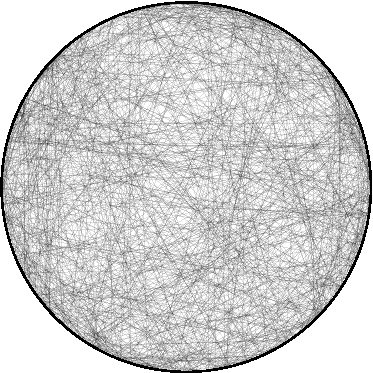
\includegraphics[keepaspectratio]{quiz_solutions_files/figure-latex/unnamed-chunk-7-1.pdf}}

This seems pretty much uniform, so let us also check the other two
approaches. We now sample random chords by picking their midpoints at
random and then computing the chord edges.

\begin{Shaded}
\begin{Highlighting}[]
\CommentTok{\# Midpoint polar coordinates}
\NormalTok{mtheta }\OtherTok{\textless{}{-}} \FunctionTok{sample}\NormalTok{(}\FunctionTok{seq}\NormalTok{(}\DecValTok{0}\NormalTok{, }\DecValTok{2}\SpecialCharTok{*}\NormalTok{pi, }\FloatTok{0.001}\NormalTok{), N, }\AttributeTok{replace =} \ConstantTok{TRUE}\NormalTok{)}
\CommentTok{\# There is a whole lot to explain about why we take square roots here...}
\NormalTok{mr }\OtherTok{\textless{}{-}} \FunctionTok{sqrt}\NormalTok{(}\FunctionTok{sample}\NormalTok{(}\FunctionTok{seq}\NormalTok{(}\DecValTok{0}\NormalTok{, }\DecValTok{1}\NormalTok{, }\FloatTok{0.001}\NormalTok{), N, }\AttributeTok{replace =} \ConstantTok{TRUE}\NormalTok{))}
\CommentTok{\# Vectorised operations to speed up execution}
\NormalTok{cs }\OtherTok{\textless{}{-}} \FunctionTok{cos}\NormalTok{(mtheta)}
\NormalTok{ss }\OtherTok{\textless{}{-}} \FunctionTok{sin}\NormalTok{(mtheta)}
\NormalTok{my }\OtherTok{\textless{}{-}} \FunctionTok{sqrt}\NormalTok{(}\DecValTok{1} \SpecialCharTok{{-}}\NormalTok{ mr}\SpecialCharTok{\^{}}\DecValTok{2}\NormalTok{)}
\NormalTok{chords }\OtherTok{\textless{}{-}} \FunctionTok{list}\NormalTok{()}
\ControlFlowTok{for}\NormalTok{ (i }\ControlFlowTok{in} \DecValTok{1}\SpecialCharTok{:}\NormalTok{N) \{}
\NormalTok{  a }\OtherTok{\textless{}{-}} \FunctionTok{c}\NormalTok{(mr[i], my[i])}
\NormalTok{  b }\OtherTok{\textless{}{-}} \FunctionTok{c}\NormalTok{(mr[i], }\SpecialCharTok{{-}}\NormalTok{my[i])}
\NormalTok{  rot }\OtherTok{\textless{}{-}} \FunctionTok{matrix}\NormalTok{(}\FunctionTok{c}\NormalTok{(cs[i], ss[i], }\SpecialCharTok{{-}}\NormalTok{ss[i], cs[i]), }\AttributeTok{nrow =} \DecValTok{2}\NormalTok{, }\AttributeTok{ncol =} \DecValTok{2}\NormalTok{, }\AttributeTok{byrow =} \ConstantTok{TRUE}\NormalTok{)}
\NormalTok{  ra }\OtherTok{\textless{}{-}}\NormalTok{ rot }\SpecialCharTok{\%*\%}\NormalTok{ a}
\NormalTok{  rb }\OtherTok{\textless{}{-}}\NormalTok{ rot }\SpecialCharTok{\%*\%}\NormalTok{ b}
\NormalTok{  chords[[i]] }\OtherTok{\textless{}{-}} \FunctionTok{list}\NormalTok{(}\FunctionTok{c}\NormalTok{(ra[}\DecValTok{1}\NormalTok{], rb[}\DecValTok{1}\NormalTok{]), }\FunctionTok{c}\NormalTok{(ra[}\DecValTok{2}\NormalTok{], rb[}\DecValTok{2}\NormalTok{]))}
\NormalTok{\}}
\CommentTok{\# Draw chords}
\FunctionTok{draw\_chords}\NormalTok{(chords)}
\end{Highlighting}
\end{Shaded}

\pandocbounded{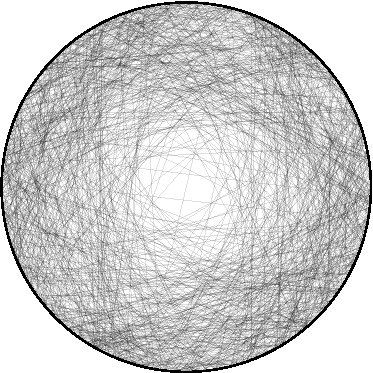
\includegraphics[keepaspectratio]{quiz_solutions_files/figure-latex/unnamed-chunk-8-1.pdf}}

Okay, this seems less uniform than the previous one. Let us also explore
the third approach:

\begin{Shaded}
\begin{Highlighting}[]
\CommentTok{\# Midpoint polar coordinates}
\NormalTok{mtheta }\OtherTok{\textless{}{-}} \FunctionTok{sample}\NormalTok{(}\FunctionTok{seq}\NormalTok{(}\DecValTok{0}\NormalTok{, }\DecValTok{2}\SpecialCharTok{*}\NormalTok{pi, }\FloatTok{0.001}\NormalTok{), N, }\AttributeTok{replace =} \ConstantTok{TRUE}\NormalTok{)}
\NormalTok{mr }\OtherTok{\textless{}{-}} \FunctionTok{sample}\NormalTok{(}\FunctionTok{seq}\NormalTok{(}\DecValTok{0}\NormalTok{, }\DecValTok{1}\NormalTok{, }\FloatTok{0.001}\NormalTok{), N, }\AttributeTok{replace =} \ConstantTok{TRUE}\NormalTok{)}
\CommentTok{\# Vectorised operations to speed up execution}
\NormalTok{cs }\OtherTok{\textless{}{-}} \FunctionTok{cos}\NormalTok{(mtheta)}
\NormalTok{ss }\OtherTok{\textless{}{-}} \FunctionTok{sin}\NormalTok{(mtheta)}
\NormalTok{my }\OtherTok{\textless{}{-}} \FunctionTok{sqrt}\NormalTok{(}\DecValTok{1} \SpecialCharTok{{-}}\NormalTok{ mr}\SpecialCharTok{\^{}}\DecValTok{2}\NormalTok{)}
\NormalTok{chords }\OtherTok{\textless{}{-}} \FunctionTok{list}\NormalTok{()}
\ControlFlowTok{for}\NormalTok{ (i }\ControlFlowTok{in} \DecValTok{1}\SpecialCharTok{:}\NormalTok{N) \{}
\NormalTok{  a }\OtherTok{\textless{}{-}} \FunctionTok{c}\NormalTok{(mr[i], my[i])}
\NormalTok{  b }\OtherTok{\textless{}{-}} \FunctionTok{c}\NormalTok{(mr[i], }\SpecialCharTok{{-}}\NormalTok{my[i])}
\NormalTok{  rot }\OtherTok{\textless{}{-}} \FunctionTok{matrix}\NormalTok{(}\FunctionTok{c}\NormalTok{(cs[i], ss[i], }\SpecialCharTok{{-}}\NormalTok{ss[i], cs[i]), }\AttributeTok{nrow =} \DecValTok{2}\NormalTok{, }\AttributeTok{ncol =} \DecValTok{2}\NormalTok{, }\AttributeTok{byrow =} \ConstantTok{TRUE}\NormalTok{)}
\NormalTok{  ra }\OtherTok{\textless{}{-}}\NormalTok{ rot }\SpecialCharTok{\%*\%}\NormalTok{ a}
\NormalTok{  rb }\OtherTok{\textless{}{-}}\NormalTok{ rot }\SpecialCharTok{\%*\%}\NormalTok{ b}
\NormalTok{  chords[[i]] }\OtherTok{\textless{}{-}} \FunctionTok{list}\NormalTok{(}\FunctionTok{c}\NormalTok{(ra[}\DecValTok{1}\NormalTok{], rb[}\DecValTok{1}\NormalTok{]), }\FunctionTok{c}\NormalTok{(ra[}\DecValTok{2}\NormalTok{], rb[}\DecValTok{2}\NormalTok{]))}
\NormalTok{\}}
\CommentTok{\# Draw chords}
\FunctionTok{draw\_chords}\NormalTok{(chords)}
\end{Highlighting}
\end{Shaded}

\pandocbounded{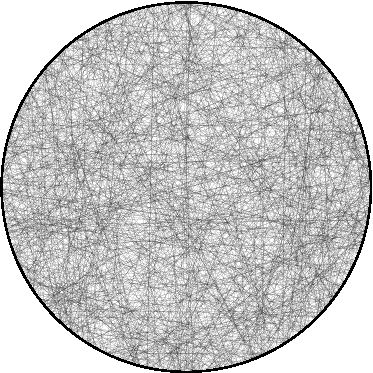
\includegraphics[keepaspectratio]{quiz_solutions_files/figure-latex/unnamed-chunk-9-1.pdf}}

This looks like the most uniform.

But, all those are just simulations to get an intuition. The original
view of Bertrand (and many other mathematicians), is that we cannot
actually pick a correct formulation and make any calculations the way
the problem has been posed, because it is ill-defined, i.e., the setting
itself is not clear enough to guide us through the process. Thus, all of
the above approaches (and results) are equally good (or bad).

The point of all this is to be careful with how things are described
within a particular probabilistic setting!

\end{document}
